% !TEX root = ../slides_ISSTA.tex
\subsection{Behavioral Clustering}
\begin{frame}
\frametitle{Part 3}

\begin{block}{RQ4}
How behaviorally similar are regexes across projects?
\end{block}
\end{frame}

%{
%\setbeamertemplate{background canvas}{\tikz[remember picture]\node[opacity=0.7] at (current page.center) {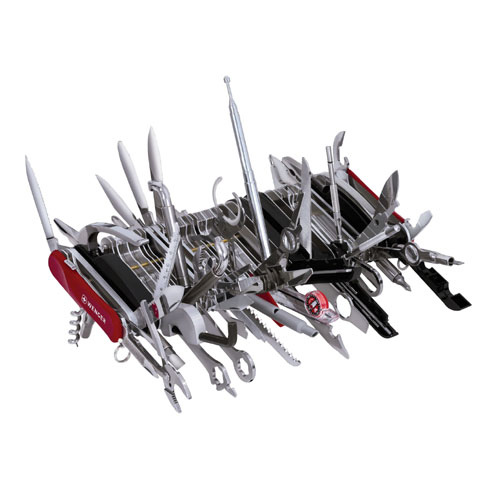
\includegraphics[keepaspectratio]{nontex/illustrations/swissArmyMess.jpg}};}
%\begin{frame}
%\frametitle{What Are Regexes Used For?}
%
%\begin{block}{\begin{Large}Non-Anecdotal Knowledge About Usage Is Missing\end{Large}}
%\begin{itemize}
%\item \begin{large}task categories\end{large}
%\item \begin{large}behavioral categories\end{large}
%\end{itemize}
%\end{block}
%\end{frame}
%}
%\note[itemize]{
%\item modern agile techniques focus on user stories and use cases - designing around anecdotal knowledge is the norm for regex
%}

%------------------------------------------------

%\begin{frame}
%\frametitle{Why do developers use regexes?}
%
%\begin{block}{RQ4}
%How behaviorally similar are regexes across projects?
%\end{block}
%\end{frame}

\begin{frame}
\frametitle{How to find common behaviors?}
\begin{enumerate}
\item \sout{thorough inspection of 53K utilizations}
\item \sout{cluster by syntactic similarity like Jaccard or longest substring}
\item \sout{formal analytical subsumption, no sufficient tools at the moment}
%\item \sout{formal analytical subsumption, using brics (30\% or less)}
\item \begin{Large}Chosen technique: cluster by behavioral similarity using Rex \end{Large}
\end{enumerate}
\end{frame}
\note[itemize]{
    \item has2: 4694
    \item hampi:
    \item bricsOK: 1415? 30\% or less
    \item rexOK-actual: 2871 61\%
}

%------------------------------------------------


\begin{frame}[fragile]
\frametitle{Example}

\begin{Large}
\begin{columns}

\begin{column}{0.4\textwidth}
\begin{itemize}
\item[A] \cverb!(ab*c|yz*)$!
	\begin{itemize}
		\item abbbbbbbc	
		\item y
		\item abcy	
		\item pac
		\item abcyzzz
	\end{itemize}
\end{itemize}

\onslide<2->{A matches 3/5 = 60\% of B's strings}

\end{column}

\begin{column}{0.4\textwidth}
\begin{itemize}
	\item[B] \cverb!(ab*c|yz*)!
	\begin{itemize}
		\item y
		\item abc
		\item abcy	
		\item  {abcccc }
		\item {yxw}
	\end{itemize}
	
	\end{itemize}
	
\onslide<3->{B matches 5/5 = 100\% of A's strings}	
	
\end{column}
\end{columns}

\onslide<4-> 
\begin{block}{}
\begin{center}
A and B are 80\% similar
\end{center}
\end{block}
\end{Large}
\end{frame}


\begin{frame}
\frametitle{Similarity Matrix $\rightarrow$ MCL}
%\begin{figure}[ht]
%  \centering
%  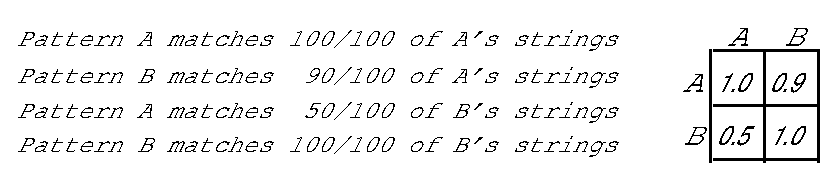
\includegraphics[scale=0.65]{nontex/illustrations/minimalMatrix.eps}
%  \label{fig:minimalMatrix}
%\end{figure}

\begin{columns}[t] % The "c" option specifies centered vertical alignment while the "t" option is used for top vertical alignment
\column{.6\textwidth} % Left column and width
\begin{figure}[h]
  \centering
  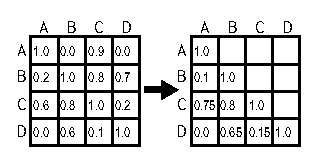
\includegraphics[scale=1]{nontex/illustrations/matrixToGraph.eps}
  \label{fig:matrixToGraph}
\end{figure}
\column{.4\textwidth} % Right column and width
\begin{center}
Rex  generates \\
400 strings for each regex.\\
Average scores to half-matrix for MCL\\
\end{center}
\end{columns}
\end{frame}



\note[itemize]{
    \item ok, simple
}





%------------------------------------------------

%\begin{frame}
%\frametitle{MCL example}
%\begin{figure}[ht]
%  \centering
%  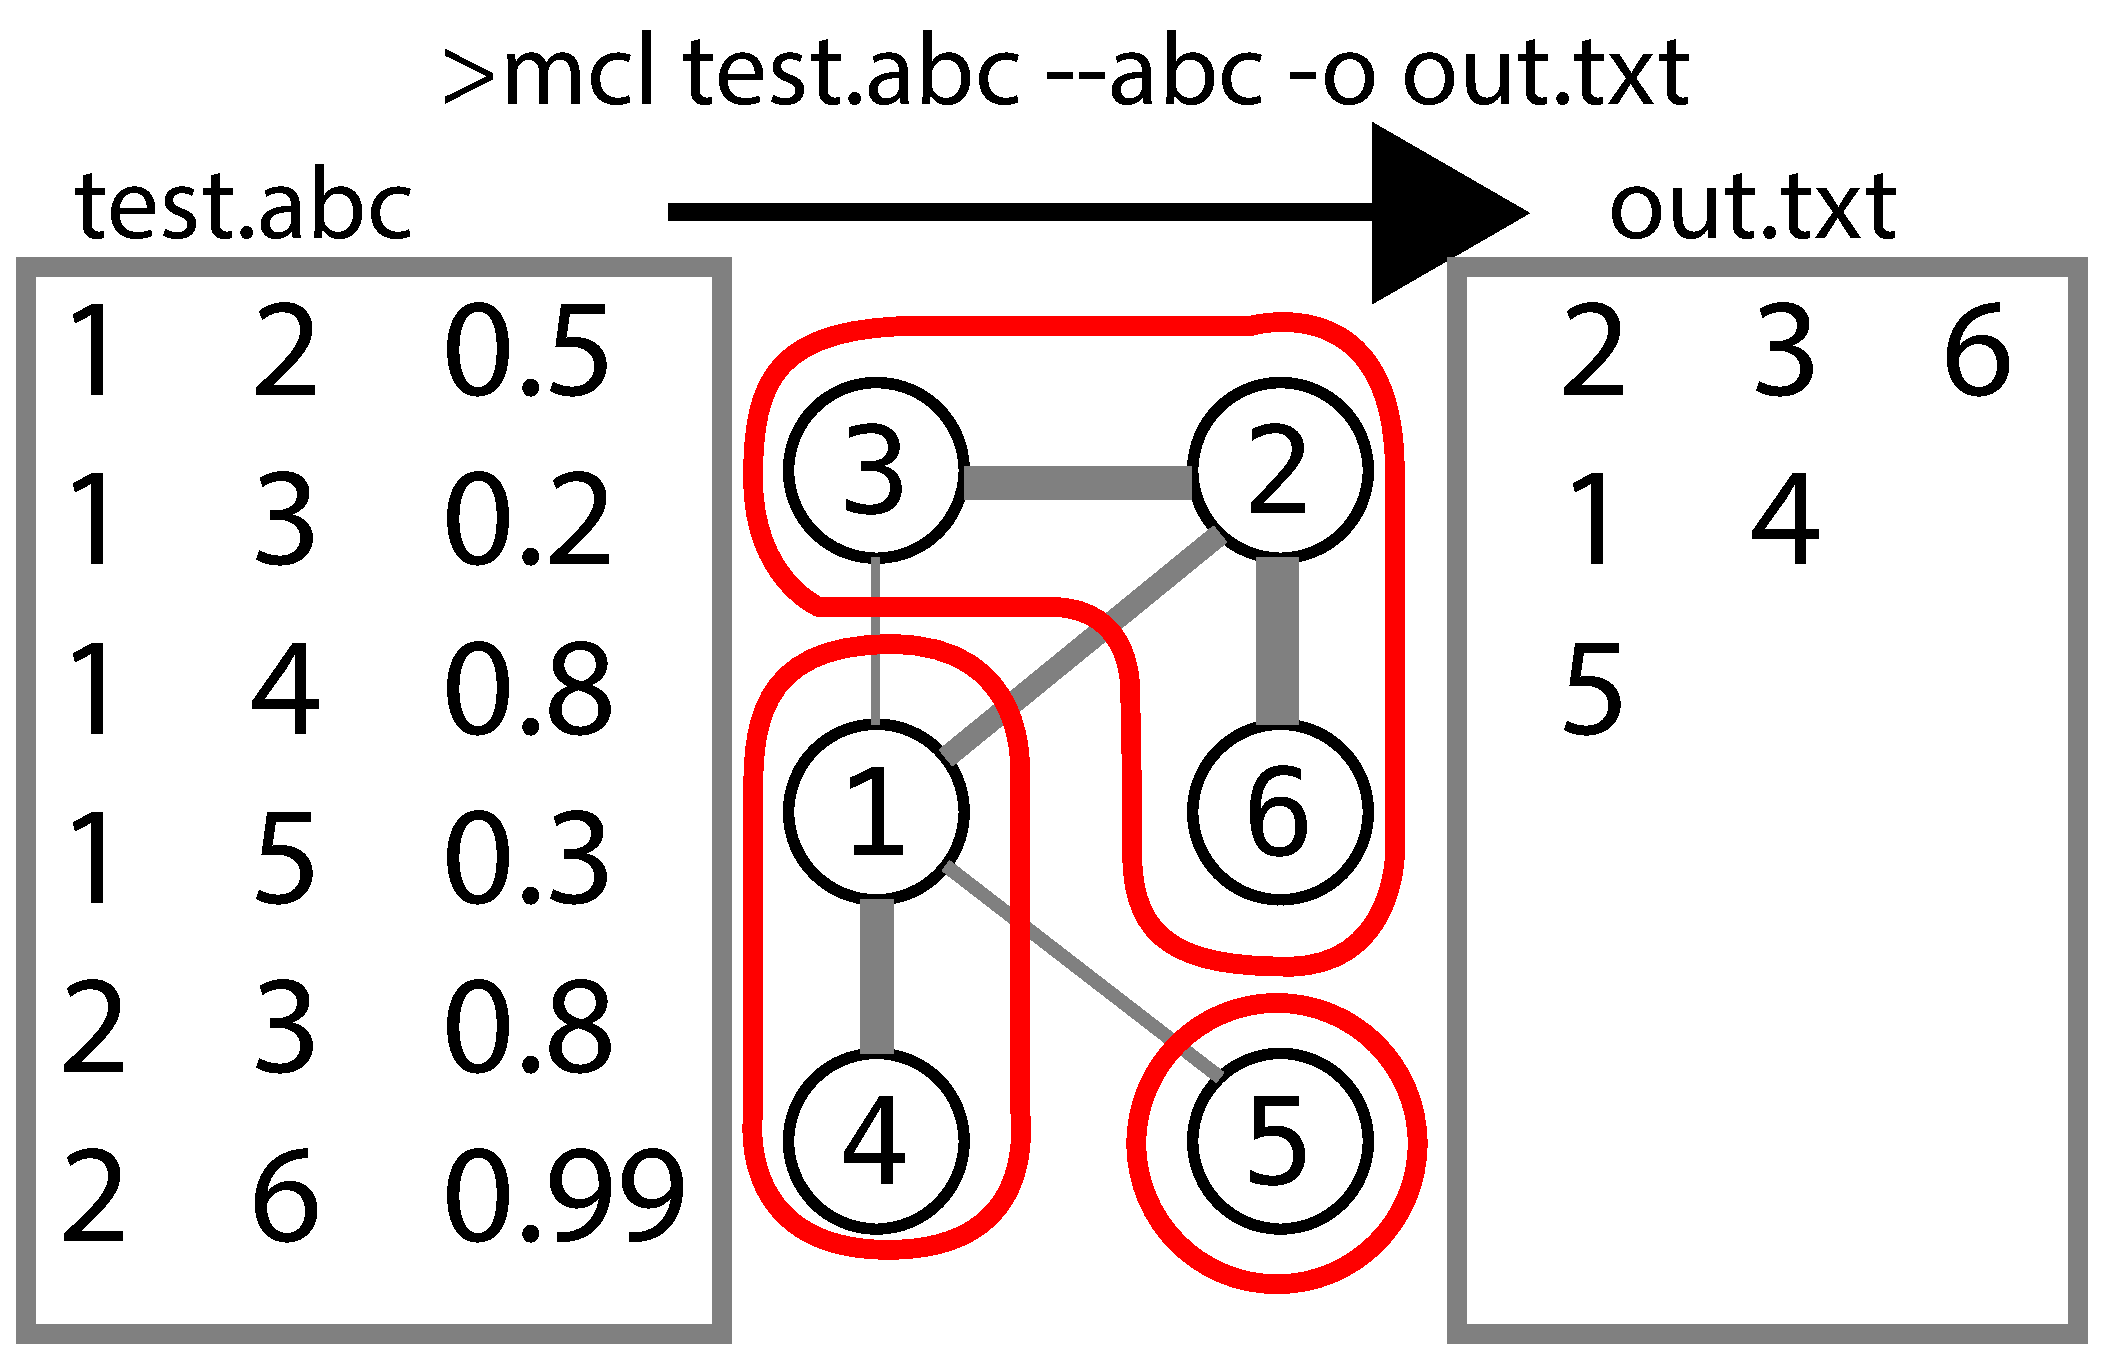
\includegraphics[scale=0.24]{nontex/illustrations/mclExample.eps}
%  \label{fig:mclExample}
%\end{figure}
%mcl works by alternating between expansion and inflation (\cite{mcl})
%\end{frame}
%\note[itemize]{
%    \item has2: 4694
%    \item bricsOK: 1415? 30\% or less
%    \item rexOK-actual: 2871 61\%
%}

%------------------------------------------------

%note here are are interested in cross-project similarity
\begin{frame}
\frametitle{Scope}

\begin{itemize}
\item 3,582 (26\%) of patterns appeared in multiple projects 
\item 711 unsupported by Rex
\vspace{12pt}
\item<2-> 2,871 patterns analyzed from 722 (44\%) of the projects
\end{itemize}

\end{frame}

\begin{frame}[fragile]
\frametitle{Clustering Results}
\onslide<2->{
\begin{center}
Example Cluster
\end{center}

\begin{table}
\begin{center}
\caption{An example cluster containing 12 regexes, with at least one regex present in 31 different projects.  In this cluster, every regex requires `:'.}
\label{table:exampleCluster}
\begin{small}
\begin{tabular}
{lcc | lcc}
\toprule \bigstrut
\textbf{Index} & \textbf{Pattern} & \textbf{NProjects} & \textbf{Index} & \textbf{Pattern} & \textbf{NProjects} \\
 \midrule \bigstrut
1 & \begin{minipage}{1.6in}\cverb!\s*([^: ]*)\s*:(.*)!\end{minipage} & 9 & 7 & \begin{minipage}{1.6in}\cverb![:]!\end{minipage} & 6 \\
 \midrule \bigstrut
2 & \begin{minipage}{1.6in}\cverb!:+!\end{minipage} & 8 & 8 & \begin{minipage}{1.6in}\cverb!([^:]+):(.*)!\end{minipage} & 6 \\
 \midrule \bigstrut
3 & \begin{minipage}{1.6in}\cverb!(:)!\end{minipage} & 8 & 9 & \begin{minipage}{1.6in}\cverb!\s*:\s*!\end{minipage} & 4 \\
 \midrule \bigstrut
4 & \begin{minipage}{1.6in}\cverb!(:+)!\end{minipage} & 8 & 10 & \begin{minipage}{1.6in}\cverb!\:!\end{minipage} & 2 \\
 \midrule \bigstrut
5 & \begin{minipage}{1.6in}\cverb!(:)(:*)!\end{minipage} & 8 & 11 & \begin{minipage}{1.6in}\cverb!^([^:]*):[^:]*$!\end{minipage} & 2 \\
 \midrule \bigstrut
6 & \begin{minipage}{1.6in}\cverb!^([^:]*): *(.*)!\end{minipage} & 8 & 12 & \begin{minipage}{1.6in}\cverb!^[^:]*:([^:]*)$!\end{minipage} & 2 \\
\bottomrule
\end{tabular}
\vspace{-6pt}
\end{small}
\end{center}
\vspace{-12pt}
\end{table}

\begin{center}
}
From 2,871 distinct regexes:
\\$\rightarrow$ 186 clusters with size $\geq$ 2
\\$\rightarrow$ 2,042 unclustered regexes
\end{center}
\end{frame}

\note[itemize]{
    \item has2: 4694
    \item bricsOK: 1415? 30\% or less
    \item rexOK-actual: 2871 61\%
}

%------------------------------------------------


\begin{frame}[fragile]
\frametitle{Six Categories Of Clusters}
\begin{table}
\begin{center}
\begin{small}
\caption{Cluster categories and sizes, ordered by number of projects containing at least one pattern in the category. \label{tab:clustercats}}
\begin{tabular}{lcccc}
\toprule
\textbf{Category} & \textbf{Clusters} & \textbf{Patterns} & \textbf{Projects} & \textbf{\% Projects} \\  \midrule \bigstrut
Multi Matches & 21 & 237 & 295 & 40\% \\
\midrule \bigstrut
Specific Char & 17 & 103 & 184 & 25\% \\
\midrule \bigstrut
Anchored Patterns & 20 & 85 & 141 & 19\% \\
\midrule \bigstrut
Two or More Chars & 16 & 40 & 120 & 16\% \\
\midrule \bigstrut
Content of Parens & 10 & 46 & 111 & 15\% \\
\midrule \bigstrut
Code Search & 15 & 27 & 92 & 13\% \\
\bottomrule
\end{tabular}
\vspace{-12pt}
\end{small}
\end{center}
\end{table}

\begin{columns}[b]
\column{.5\textwidth}
\begin{footnotesize}
\begin{description}
\item [Multi Matches] \cverb!(\s)!, \cverb!,|;!
\item [Specific Char] \cverb!:+!, \cverb!}!, \cverb!%!
\item [Anchored Patterns] \cverb!^[-_A-Za-z0-9]+$!
\end{description}
\end{footnotesize}
\column{.5\textwidth}
\begin{footnotesize}
\begin{description}
\item [Two Or More Chars] \cverb!@[a-z]+!
\item [Content of Parens] \cverb!<(.+)>!, \cverb!<[^>]*?>!
\item [Code Search]\cverb!.*rlen=([0-9]+)!
\end{description}
\end{footnotesize}
\end{columns}
\end{frame}
\note[itemize]{
    \item partially successful
    \item did identify some use cases
    \item technique ignores 39\%
    \item technique fails to cluster similar intent, similar syntax, similar rules, labels, etc.
}



\begin{frame}
\frametitle{Notable Observations}

\begin{block}{}
\begin{itemize}
	\item Finding a specific character is quite common, 25\% of projects (in contrast with survey)
	\item Regexes are often used to parse source code!
\end{itemize}
\end{block}

\onslide<2->
but....

\onslide<3->
\begin{block}{}
\begin{itemize}
	\item Similarity metric is approximate
	\item Metric is perhaps \emph{too} sensitive to differences in literals
\end{itemize}
\end{block}

%\onslide<4->
%More importantly,
%
%\onslide<5->
%\begin{block}{}
%What's the bigger picture?
%\end{block}


\end{frame}

%------------------------------------------------
